\documentclass{article}

\usepackage{arxiv}

\usepackage[utf8]{inputenc} % allow utf-8 input
\usepackage[T1]{fontenc}    % use 8-bit T1 fonts
\usepackage{lmodern}        % https://github.com/rstudio/rticles/issues/343
\usepackage{hyperref}       % hyperlinks
\usepackage{url}            % simple URL typesetting
\usepackage{booktabs}       % professional-quality tables
\usepackage{amsfonts}       % blackboard math symbols
\usepackage{nicefrac}       % compact symbols for 1/2, etc.
\usepackage{microtype}      % microtypography
\usepackage{graphicx}

\title{Great Britain Accessibility Indicators 2023: Data descriptor}

\author{
    J Rafael Verduzco-Torres
   \\
    Urban Big Data Centre \\
    University of Glasgow \\
  Glasgow, G12 8RZ \\
  \texttt{\href{mailto:JoseRafael.Verduzco-Torres@glasgow.ac.uk}{\nolinkurl{JoseRafael.Verduzco-Torres@glasgow.ac.uk}}} \\
   \And
    David P McArthur
   \\
    Urban Big Data Centre \\
    University of Glasgow \\
  Glasgow, G12 8RZ \\
  \texttt{\href{mailto:David.Mcarthur@glasgow.ac.uk}{\nolinkurl{David.Mcarthur@glasgow.ac.uk}}} \\
  }


% tightlist command for lists without linebreak
\providecommand{\tightlist}{%
  \setlength{\itemsep}{0pt}\setlength{\parskip}{0pt}}


% Pandoc citation processing
\newlength{\cslhangindent}
\setlength{\cslhangindent}{1.5em}
\newlength{\csllabelwidth}
\setlength{\csllabelwidth}{3em}
\newlength{\cslentryspacingunit} % times entry-spacing
\setlength{\cslentryspacingunit}{\parskip}
% for Pandoc 2.8 to 2.10.1
\newenvironment{cslreferences}%
  {}%
  {\par}
% For Pandoc 2.11+
\newenvironment{CSLReferences}[2] % #1 hanging-ident, #2 entry spacing
 {% don't indent paragraphs
  \setlength{\parindent}{0pt}
  % turn on hanging indent if param 1 is 1
  \ifodd #1
  \let\oldpar\par
  \def\par{\hangindent=\cslhangindent\oldpar}
  \fi
  % set entry spacing
  \setlength{\parskip}{#2\cslentryspacingunit}
 }%
 {}
\usepackage{calc}
\newcommand{\CSLBlock}[1]{#1\hfill\break}
\newcommand{\CSLLeftMargin}[1]{\parbox[t]{\csllabelwidth}{#1}}
\newcommand{\CSLRightInline}[1]{\parbox[t]{\linewidth - \csllabelwidth}{#1}\break}
\newcommand{\CSLIndent}[1]{\hspace{\cslhangindent}#1}

\usepackage{amsmath}
\usepackage{booktabs}
\usepackage{longtable}
\usepackage{array}
\usepackage{multirow}
\usepackage{wrapfig}
\usepackage{float}
\usepackage{colortbl}
\usepackage{pdflscape}
\usepackage{tabu}
\usepackage{threeparttable}
\usepackage{threeparttablex}
\usepackage[normalem]{ulem}
\usepackage{makecell}
\usepackage{xcolor}
\begin{document}
\maketitle


\begin{abstract}
The dataset described in this paper introduces a suite of updated
accessibility indicators to key services for Great Britain (Great
Britain Accessibility Indicators 2023, AI23), expanding on the previous
Public Transport Accessibility Indicators (PTAI22). AI23 enhances
previous versions by incorporating walking and cycling modes,
disaggregating employment accessibility by industry, adding pharmacies,
parks and gardens, and extending public transport estimates to evening
off-peak times. AI23 facilitates seamless integration into varied
analyses given the use of small-area official geographies.
\end{abstract}

\keywords{
    Accessibility
   \and
    Transport
   \and
    Active travel
   \and
    Health
   \and
    Employment
  }

\hypertarget{background-summary}{%
\section{Background \& Summary}\label{background-summary}}

Accessibility indicators measure the ease of reaching valuable
destinations (Levinson and Wu 2020). The current dataset, Great Britain
Accessibility Indicators 2023 (AI23), provides small-area indicators to
key services such as health, education, employment, and urban centres.
This dataset is an updated and expanded version of the the Public
Transport Accessibility Indicators for Great Britain 2022 (PTAI22)
dataset described here: \url{https://zenodo.org/records/6759240}
(Verduzco Torres and McArthur 2022).

The data described here represent a snapshot from the first quarter of
2023, whereas the PTAI22 corresponds to the last quarter of 2021. Where
applicable, the AI23 indicators are directly comparable with the
previous version. The AI23 has been expanded from the PTAI22 in the
following ways:

\begin{itemize}
\tightlist
\item
  It includes active modes, specifically walking and cycling, in
  addition to public transport.
\item
  Accessibility to employment is now disaggregated by the UK Standard
  Industrial Classification of Economic Activities (UK SIC).
\item
  Pharmacies have been added as an additional health destination in the
  AI23 dataset.
\item
  Public parks and gardens are included as a main recreational service.
\item
  The public transport indicators now cover not only the morning peak
  but also the evening off-peak period.
\end{itemize}

In particular, the current dataset provides a suite of ready-to-use
accessibility indicators to key services such as employment, general
practices (GPs), hospitals, pharmacies, parks and gardens, primary and
secondary schools, supermarkets, main urban centres, and urban
sub-centres. These indicators are available for 42,000 small area units
across Great Britain, specifically at the Lower Super Output Area (LSOA)
level in England and Wales, and the Data Zone (DZ) level in Scotland.

Accessibility indicators have been used in research to examine a broad
array of regional and urban issues, including unemployment rates in the
labour market (Bastiaanssen, Johnson, and Lucas 2022), vaccination
uptake in public health (Chen et al. 2023), and residential property
prices (Verduzco Torres 2023a). Similarly, their relevance in planning
and policymaking is increasing, serving as input for developing
comprehensive project appraisals (Cavallaro, Bruzzone, and Nocera 2023),
conducting 20-minute neighbourhood analyses, and as a performance
benchmark.

\hypertarget{methods}{%
\section{Methods}\label{methods}}

The methods and sources used for the current dataset largely follow
those outlined in the previous version
(\url{https://zenodo.org/records/6759240}) (Verduzco Torres and McArthur
2022). The remainder of the paper focuses on the key aspects and
extensions unique to this version.

The accessibility indicators, denoted as \(A\), are constructed using
location-based measures, which encompass cumulative, relative
cumulative, and dual or nearest opportunity measures. These
location-based measures are calculated from an origin point \(i\) and
take into account the type of opportunity \(W_k\) at potential
destinations \(j\). The cumulative measures are estimated according to
the equation below.

\[
\begin{aligned}
A_{ik} &= \sum_{j=1}^{n} W_{jk} f(t_{ij}) \\
f(t_{ij}) &= \left\{
      \begin{array}{ll}
          1 & \quad \text{if }t_{ij} \leq \bar{t} \text{ (threshold value)} \\
          0 & \quad \text{otherwise}.
      \end{array}
    \right.
\end{aligned}
\]

Here, it is assumed that people deem opportunities or services as
reachable if the modelled travel time between the the origin and
destination, \(t{ij}\), is equal or shorter than given threshold,
\(\bar{t}\). All services beyond this limit are disregarded. Relative
cumulative measures inputs the size of the service weighted by the total
number in the region, i.e.~\(W_{jk} / W_k\). Meanwhile, the dual or
nearest opportunity considers the minimum travel time to a destination
where the size of the service is larger that 0. In other words, these
represent the shortest travel time to the nearest facility of type
\(k\), as illustrated in the equation below.

\[
A_{ik} = \min_{j=1}^{n} \{ t_{ij} : W_{kj} > 0 \}
\]

The measures are computed using the \texttt{AccessUK} package for the
\texttt{R} language v0.0.1-alpha (Verduzco Torres 2023b).

\hypertarget{origins}{%
\subsection{Origins}\label{origins}}

The population weighted centroid of each of the 41,729 LSOA/DZ are
considered as the origins in accessibility measures measures. These
correspond to the 2011 Census (version last updated in 21 December 2019
for England and Wales, and 26 March 2021 for Scotland).

\hypertarget{key-services-at-destinations}{%
\subsection{Key services at
destinations}\label{key-services-at-destinations}}

While the indicators use the same information sources to determine the
locations of services, the most recent version available for the first
quarter of 2023 has been used, unless stated otherwise. Table 1 presents
a summary of the total number of services across the different versions
of the accessibility indicators, showing minor negative or positive
fluctuations. The data for urban centres uses the same input data.
Therefore, those figures remain unchanged.

\begin{table}[!h]

\caption{\label{tab:unnamed-chunk-2}Destionation summary}
\centering
\begin{tabu} to \linewidth {>{\raggedright}X>{\raggedright}X>{\raggedright}X}
\toprule
Destination & Total in 2022
(PTAI22) & Total in 2023
(AI23)\\
\midrule
Employment & 30 067 975 & 30 898 620\\
GPs & 7 887 & 7 756\\
Hospitals & 1 510 & 1 572\\
Parks and gardens (ha) & NA & 120 619\\
Pharmacies & NA & 12 983\\
\addlinespace
Primary schools & 19 853 & 19 830\\
Secondary schools & 3 457 & 3 466\\
Supermarkets & 6 478 & 6 392\\
Urban centre: Main & 182 & 182\\
Urban centre: Subcentre & 421 & 421\\
\bottomrule
\end{tabu}
\end{table}

\hypertarget{employment}{%
\subsubsection{Employment}\label{employment}}

In addition to accessibility to all types of employment, the AI23
dataset offers measures disaggregated by broad industrial group
according to the UK SIC (see the following URL for a detailed
description of the classification used:
\url{https://www.ons.gov.uk/methodology/classificationsandstandards/ukstandardindustrialclassificationofeconomicactivities}).
Table 2 presents the UK SIC grouping equivalence with the names used for
the accessibility indicators.

\begin{table}[!h]

\caption{\label{tab:unnamed-chunk-3}Broad industrial groups abbreviation}
\centering
\begin{tabu} to \linewidth {>{\raggedright}X>{\raggedright}X}
\toprule
Inidcator name in the IA23 & SIC broad group classification\\
\midrule
employment\_agriculture\_1 & 1 : Agriculture, forestry \& fishing (A)\\
employment\_mining\_2 & 2 : Mining, quarrying \& utilities (B,D and E)\\
employment\_manufacturing\_3 & 3 : Manufacturing (C)\\
employment\_construction\_4 & 4 : Construction (F)\\
employment\_motor\_5 & 5 : Motor trades (Part G)\\
\addlinespace
employment\_wholesale\_6 & 6 : Wholesale (Part G)\\
employment\_retail\_7 & 7 : Retail (Part G)\\
employment\_transport\_8 & 8 : Transport \& storage (inc postal) (H)\\
employment\_accommodation\_9 & 9 : Accommodation \& food services (I)\\
employment\_information\_10 & 10 : Information \& communication (J)\\
\addlinespace
employment\_financial\_11 & 11 : Financial \& insurance (K)\\
employment\_property\_12 & 12 : Property (L)\\
employment\_professional\_13 & 13 : Professional, scientific \& technical (M)\\
employment\_business\_14 & 14 : Business administration \& support services (N)\\
employment\_public\_15 & 15 : Public administration \& defence (O)\\
\addlinespace
employment\_education\_16 & 16 : Education (P)\\
employment\_health\_17 & 17 : Health (Q)\\
employment\_arts\_18 & 18 : Arts, entertainment, recreation \& other services (R,S,T and U)\\
\bottomrule
\end{tabu}
\end{table}

\hypertarget{hospitals}{%
\subsubsection{Hospitals}\label{hospitals}}

The sources and selection criterion to account for the location of
hospitals remains unchanged and uses the official updated datasets
except for Wales. In the latter case, the PTAI22 used the list of
addresses available on the Health in Wales website
(\url{http://www.wales.nhs.uk/}). However, this is no longer active.
Thus, we used the locations obtained in January 2022.

\hypertarget{parks-and-gardens}{%
\subsubsection{Parks and gardens}\label{parks-and-gardens}}

Public parks and gardens are included as recreational services. The
geolocation information is sourced from the `OS Open Greenspace' dataset
V 1.3, corresponding to April 2023 covering all of GB (available at
\url{https://www.ordnancesurvey.co.uk/products/os-open-greenspace}).
This product is licensed under the Open Government Licence, allowing the
distribution of derivative works.

The Open Greenspace dataset comprises two tables: `Greenspace Site' and
`Access Point'. The former represents the outer boundaries of
greenspaces, while the latter indicates specific entry points associated
with these boundaries. The `Greenspace Site' table was filtered to
include only geometries classified as `Public Park or Garden' in the
`function' field. Subsequently, the `Access Point' table was refined
using the linking ID from the `Greenspace Site' table.

The `Greenspace Site' polygons were overlapped onto the LSOA/DZ
geometries, with the corresponding area size in hectares (ha) being used
as the weight (\(W_{i}\)) for the service in cumulative measures. The
nearest park or garden was determined using the `Access Point'
locations. It is important to note that while the boundaries represented
in the `Greenspace Site' can indicate physical delimitations, this is
not always the case. For the purposes of this study, it is assumed that
if a polygon lacks a designated access point, entry is possible through
any point along its boundary.

\hypertarget{pharmacies}{%
\subsubsection{Pharmacies}\label{pharmacies}}

The location of pharmacies was obtained from official public health
records. The data for England comes from the `Consolidated
Pharmaceutical List' corresponding to the 2023-24 quarter 1. This was
manually downloaded from the NHS Data portal
(\url{https://opendata.nhsbsa.net/dataset/consolidated-pharmaceutical-list}).
The location of pharmacies in Scotland was accessed from the Public
Health Scotland platform. The `Dispenser Details January 2023' dataset
was downloaded from the URL:
\url{https://www.opendata.nhs.scot/dataset/dispenser-location-contact-details/resource/f44e6a10-4f1f-4ffd-9205-956944bacf95}.
The information for Wales was available from NHS website. The `Pharmacy
Chains' dataset used corresponds to June 2023 (URL:
\url{https://nwssp.nhs.wales/ourservices/primary-care-services/general-information/data-and-publications/pharmacies-in-wales/}).
These data contain address references including the postcode, which was
matched with the ONS postcode dataset to assign a corresponding LSOA/DZ
code.

\hypertarget{travel-costs}{%
\subsection{Travel costs}\label{travel-costs}}

Travel costs in the accessibility indicators \(t_{ij}\) are represented
by the modelled travel time by public transport, bicycle, and walk. The
AI23 use a series of all-to-all travel time matrices computed from each
LSOA/DZ population weighted centroids using \texttt{R5R} software
(Saraiva et al. 2021) for the \texttt{R} programming language. The main
inputs used are the OpenStreetMap road and pedestrian network, bus time
tables from Bus Open Data Service (BODS)
(\url{https://www.gov.uk/transport/bus-services-routes-and-timetables}),
and train time tables from the Rail Delivery Group
(\url{https://www.raildeliverygroup.com/}). The public transport
indicators are estimated for two times of departure, namely 7 a.m. and 9
p.m. on the 7th of March 2023, considering a three hours time window.
Additional details are offered in a separate data descriptor {[}PENDING
REFERENCE{]}.

\hypertarget{data-records}{%
\section{Data records}\label{data-records}}

The accessibility indicators can be accessed in a series of
\texttt{.csv} files from the following open-access repository:
{[}PENDING{]}. These files are organised by the type of opportunity or
service within the folder structure, and by mode within the file
nomenclature, as illustrated in the directory tree diagram provided. The
directory structure is as follows:
\texttt{root/\textless{}NAME\ OF\ SERVICE\textgreater{}/access\_\textless{}NAME\ OF\ SERVICE\textgreater{}\_\textless{}MODE\textgreater{}.csv},
with `pt' denoting public transport in the
\texttt{\textless{}MODE\textgreater{}} segment. For clarity, the diagram
does not include the disaggregated employment measures, but
\protect\hyperlink{inventory}{Appendix 1} contains a comprehensive
inventory of all files within the dataset.

\begin{verbatim}
## ../output/
## +-- employment_all
## |   +-- access_employment_all_bicycle.csv
## |   +-- access_employment_all_pt.csv
## |   \-- access_employment_all_walk.csv
## +-- gp_practices
## |   +-- access_gp_practices_bicycle.csv
## |   +-- access_gp_practices_pt.csv
## |   \-- access_gp_practices_walk.csv
## +-- hospitals
## |   +-- access_hospitals_bicycle.csv
## |   +-- access_hospitals_pt.csv
## |   \-- access_hospitals_walk.csv
## +-- inventory.csv
## +-- main_bua
## |   +-- access_main_bua_bicycle.csv
## |   +-- access_main_bua_pt.csv
## |   \-- access_main_bua_walk.csv
## +-- parks
## |   +-- access_parks_bicycle.csv
## |   +-- access_parks_pt.csv
## |   \-- access_parks_walk.csv
## +-- pharmacies
## |   +-- access_pharmacies_bicycle.csv
## |   +-- access_pharmacies_pt.csv
## |   \-- access_pharmacies_walk.csv
## +-- primary_schools
## |   +-- access_primary_schools_bicycle.csv
## |   +-- access_primary_schools_pt.csv
## |   \-- access_primary_schools_walk.csv
## +-- secondary_schools
## |   +-- access_secondary_schools_bicycle.csv
## |   +-- access_secondary_schools_pt.csv
## |   \-- access_secondary_schools_walk.csv
## +-- sub_bua
## |   +-- access_sub_bua_bicycle.csv
## |   +-- access_sub_bua_pt.csv
## |   \-- access_sub_bua_walk.csv
## +-- supermarkets
## |   +-- access_supermarkets_bicycle.csv
## |   +-- access_supermarkets_pt.csv
## |   \-- access_supermarkets_walk.csv
## \-- variable_descriptor.csv
\end{verbatim}

Table 3 presents the structure and contents of each file as outlined in
the diagram. The first column contains the 2011 Census LSOA/DZ code. The
`mode' column specifies the form of transport used to calculate the
indicators. The `time\_of\_day' column, exclusive to public transport
measures, indicates the departure time -- either `am' or `pm' -- for
which the estimates are made. The prefix `accessibility' in the column
headers denotes cumulative measures, provided across eight 15-minute
intervals ranging from 15 to 120 minutes. Relative measures are denoted
by a `pct' suffix. The column `nearest\_' shows the travel time in
minutes to the closest service of type \(k\). This column is not
applicable for employment, as these figures are aggregated from the
source.

\begin{table}[H]

\caption{\label{tab:unnamed-chunk-5}Variable descriptor}
\centering
\begin{tabu} to \linewidth {>{\raggedright}X>{\raggedright}X}
\toprule
Variable & Description\\
\midrule
geo\_code & 2011 LSOA/DZ geo-code of origin\\
mode & Mode of transport used for the indicators, values: `pt' = public transport, `bicycle', `walk'\\
time\_of\_day & Time of departure, values: `am' = 7 a.m., `pm' = 9 p.m. Available for public transport only.\\
access\_<NAME OF SERVICE>\_15 & Cumulative accessibility: Number of services of type k within 15 minutes\\
access\_<NAME OF SERVICE>\_30 & Cumulative accessibility: Number of services of type k within 30 minutes\\
\addlinespace
access\_<NAME OF SERVICE>\_45 & Cumulative accessibility: Number of services of type k within 45 minutes\\
access\_<NAME OF SERVICE>\_60 & Cumulative accessibility: Number of services of type k within 60 minutes\\
access\_<NAME OF SERVICE>\_75 & Cumulative accessibility: Number of services of type k within 75 minutes\\
access\_<NAME OF SERVICE>\_90 & Cumulative accessibility: Number of services of type k within 90 minutes\\
access\_<NAME OF SERVICE>\_105 & Cumulative accessibility: Number of services of type k within 105 minutes\\
\addlinespace
access\_<NAME OF SERVICE>\_120 & Cumulative accessibility: Number of services of type k within 120 minutes\\
access\_<NAME OF SERVICE>\_15\_pct & Relative cumulative accessibility: Number of services of type k within 15 minutes. In percent, from 0 to 100.\\
access\_<NAME OF SERVICE>\_30\_pct & Relative cumulative accessibility: Number of services of type k within 30 minutes. In percent, from 0 to 100.\\
access\_<NAME OF SERVICE>\_45\_pct & Relative cumulative accessibility: Number of services of type k within 45 minutes. In percent, from 0 to 100.\\
access\_<NAME OF SERVICE>\_60\_pct & Relative cumulative accessibility: Number of services of type k within 60 minutes. In percent, from 0 to 100.\\
\addlinespace
access\_<NAME OF SERVICE>\_75\_pct & Relative cumulative accessibility: Number of services of type k within 75 minutes. In percent, from 0 to 100.\\
access\_<NAME OF SERVICE>\_90\_pct & Relative cumulative accessibility: Number of services of type k within 90 minutes. In percent, from 0 to 100.\\
access\_<NAME OF SERVICE>\_105\_pct & Relative cumulative accessibility: Number of services of type k within 105 minutes. In percent, from 0 to 100.\\
access\_<NAME OF SERVICE>\_120\_pct & Relative cumulative accessibility: Number of services of type k within 120 minutes. In percent, from 0 to 100.\\
nearest\_<NAME OF SERVICE> & Travel time in minutes to the nearest service of type k\\
\bottomrule
\end{tabu}
\end{table}

Figure \ref{fig:access-overview} provides a visual summary of the
relative accessibility indicators to key services by mode. The
horizontal axis represents the time cut, capped at 60 minutes, while the
vertical axis displays the average relative accessibility across Great
Britain. The figure shows that public transport allows access to a
greater number of services at longer travel times (over 45 minutes).
However, for travel times less than 45 minutes, accessibility levels are
similar between bicycle and public transport, and for some services
within 30 minutes or less---such as Manufacturing (C) and Motor trades
(Part G) employment, parks, and supermarkets---accessibility is even
higher for bicycle. As expected, walking is a competitive mode only at
shorter distances.

\begin{figure}[!htbp]
  \centering
  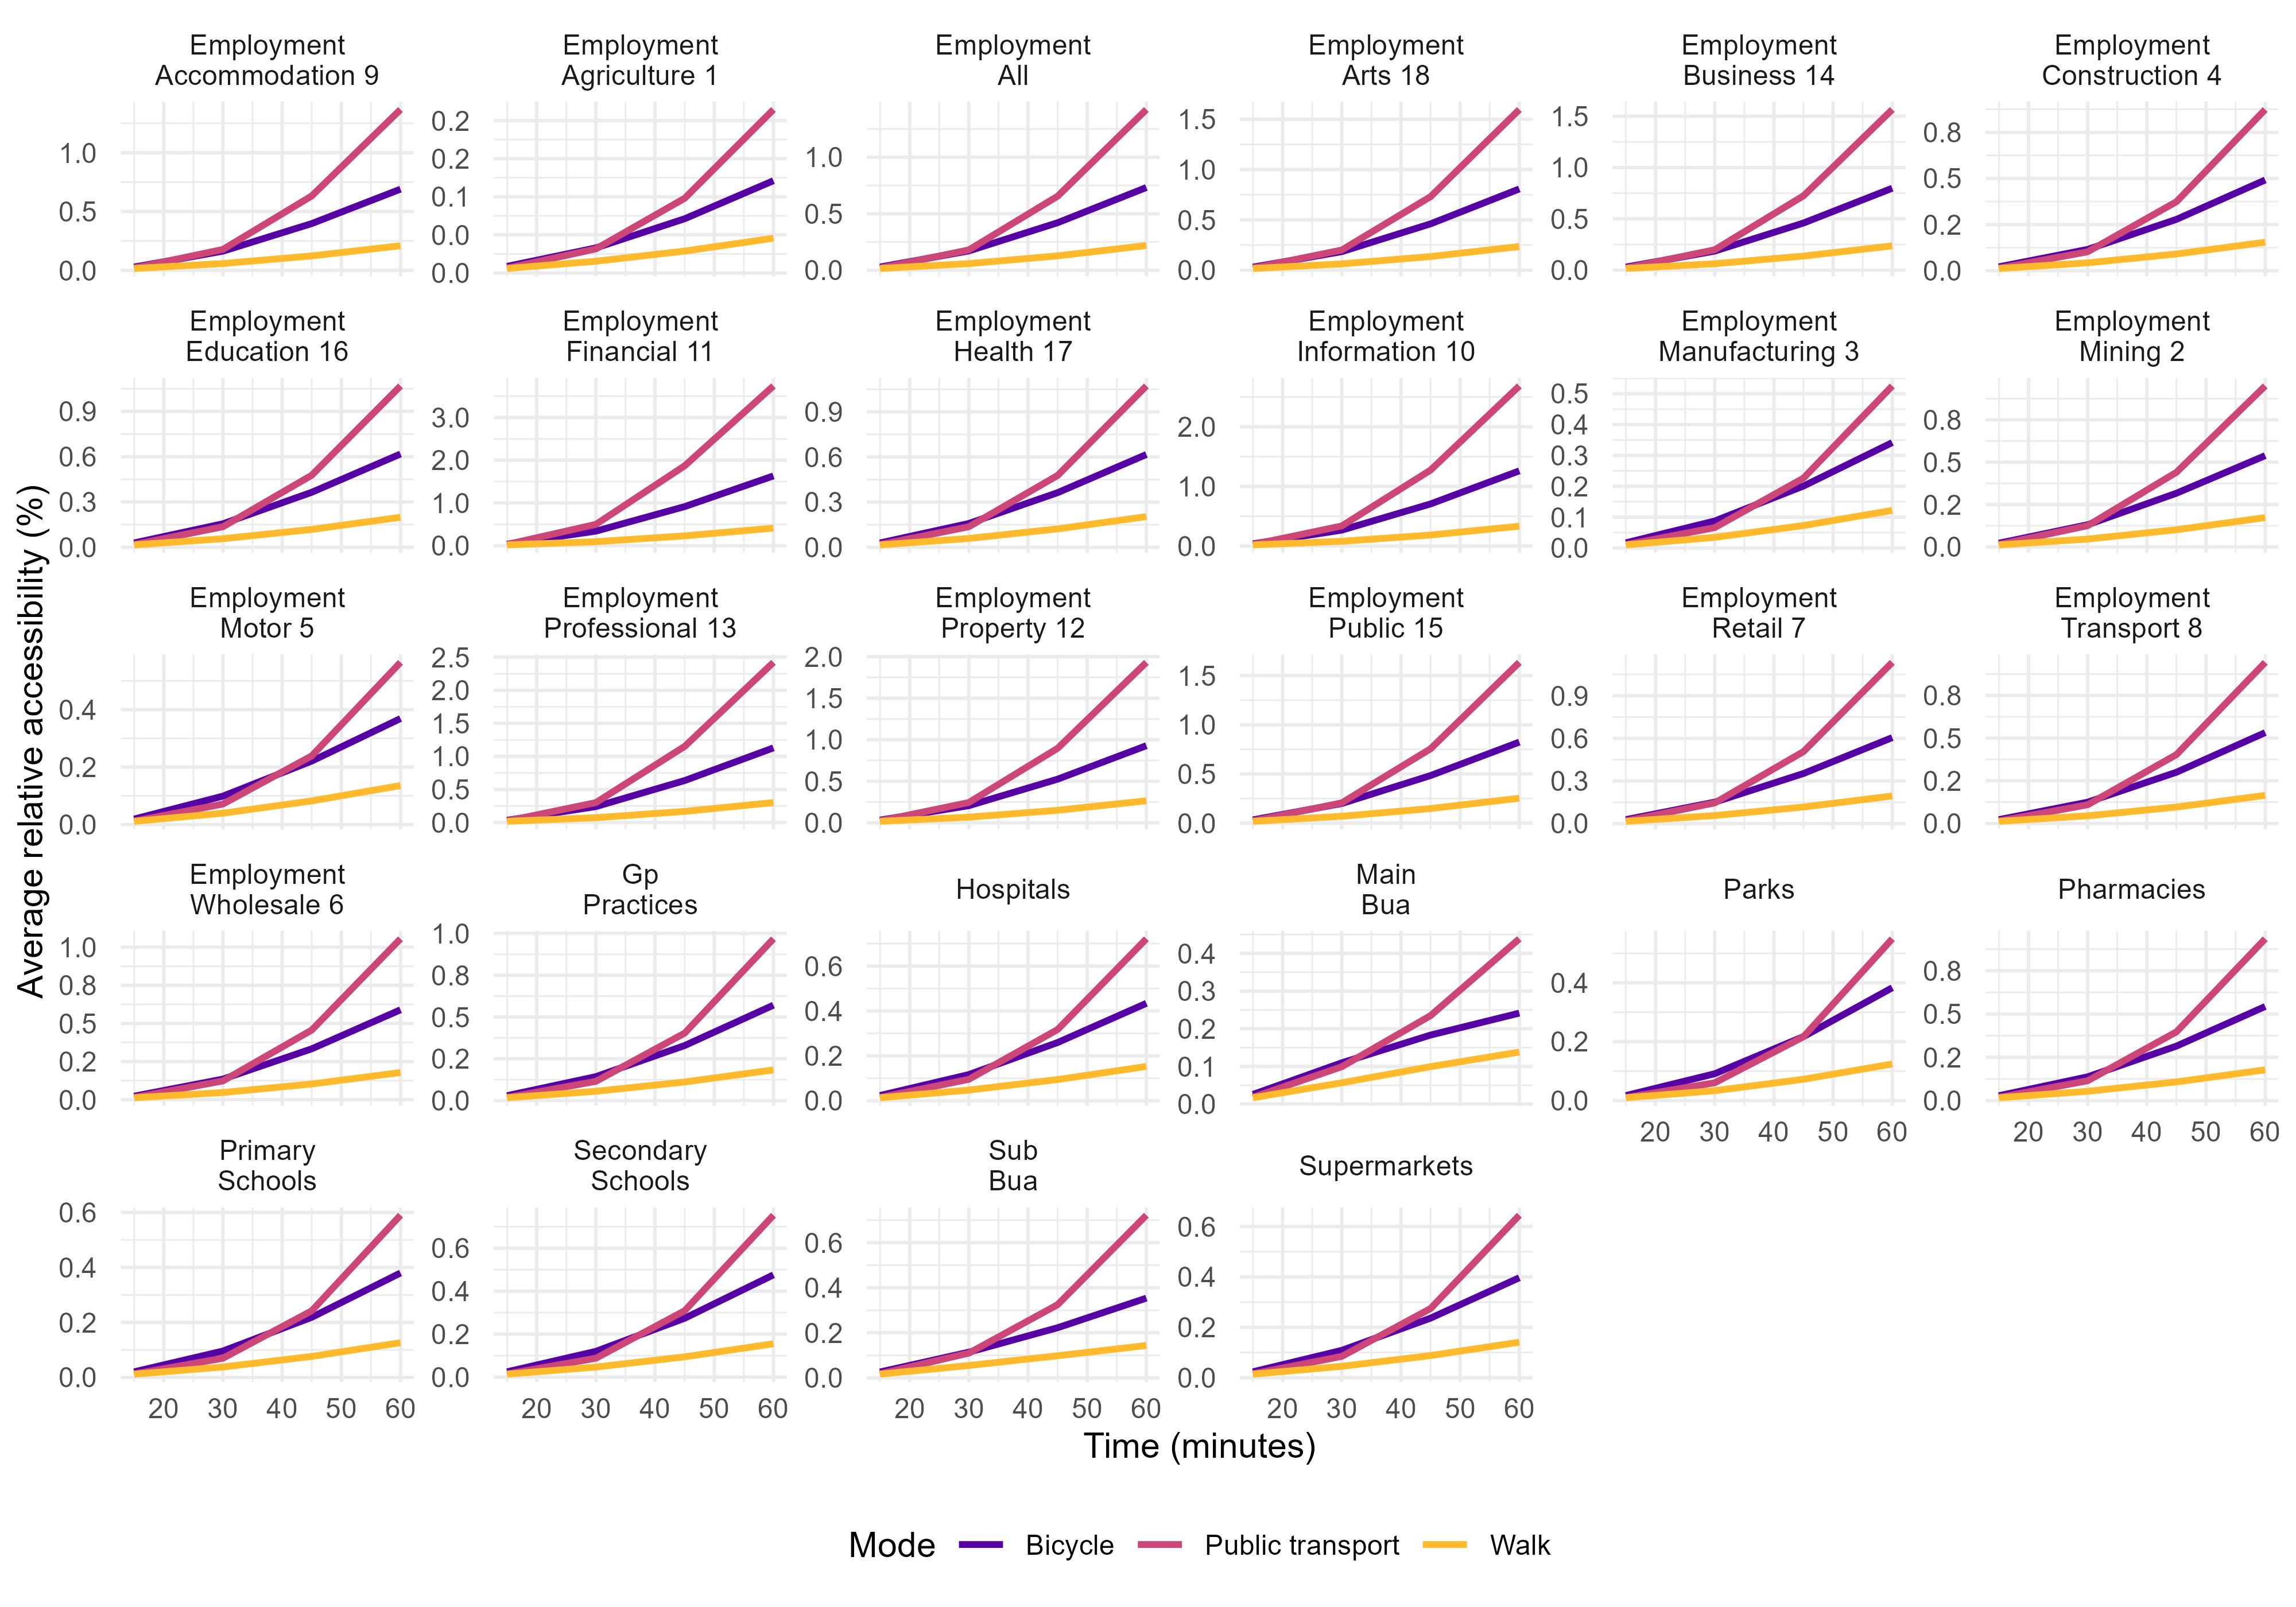
\includegraphics[width=1.0\textwidth]{../plots/line_plot_comaprison.jpg}
  \caption{Relative accessibility overview to key services for various modes.}
  \footnotesize{\textit{Source:} the author based on AI23 dataset.}
  \label{fig:access-overview}
\end{figure}

Figure \ref{fig:access-parks} illustrates the accessibility to public
parks and gardens in Greater Manchester Area within 30 minutes by
bicycle and public transport at the morning peak. The map reveals
contrasting differences. The main difference are particularly noticeable
in the south of the city. In this area, accessibility is higher by
bicycle than by public transport. Conversely, the core area has higher
access by public transport.

\begin{figure}[!htbp]
  \centering
  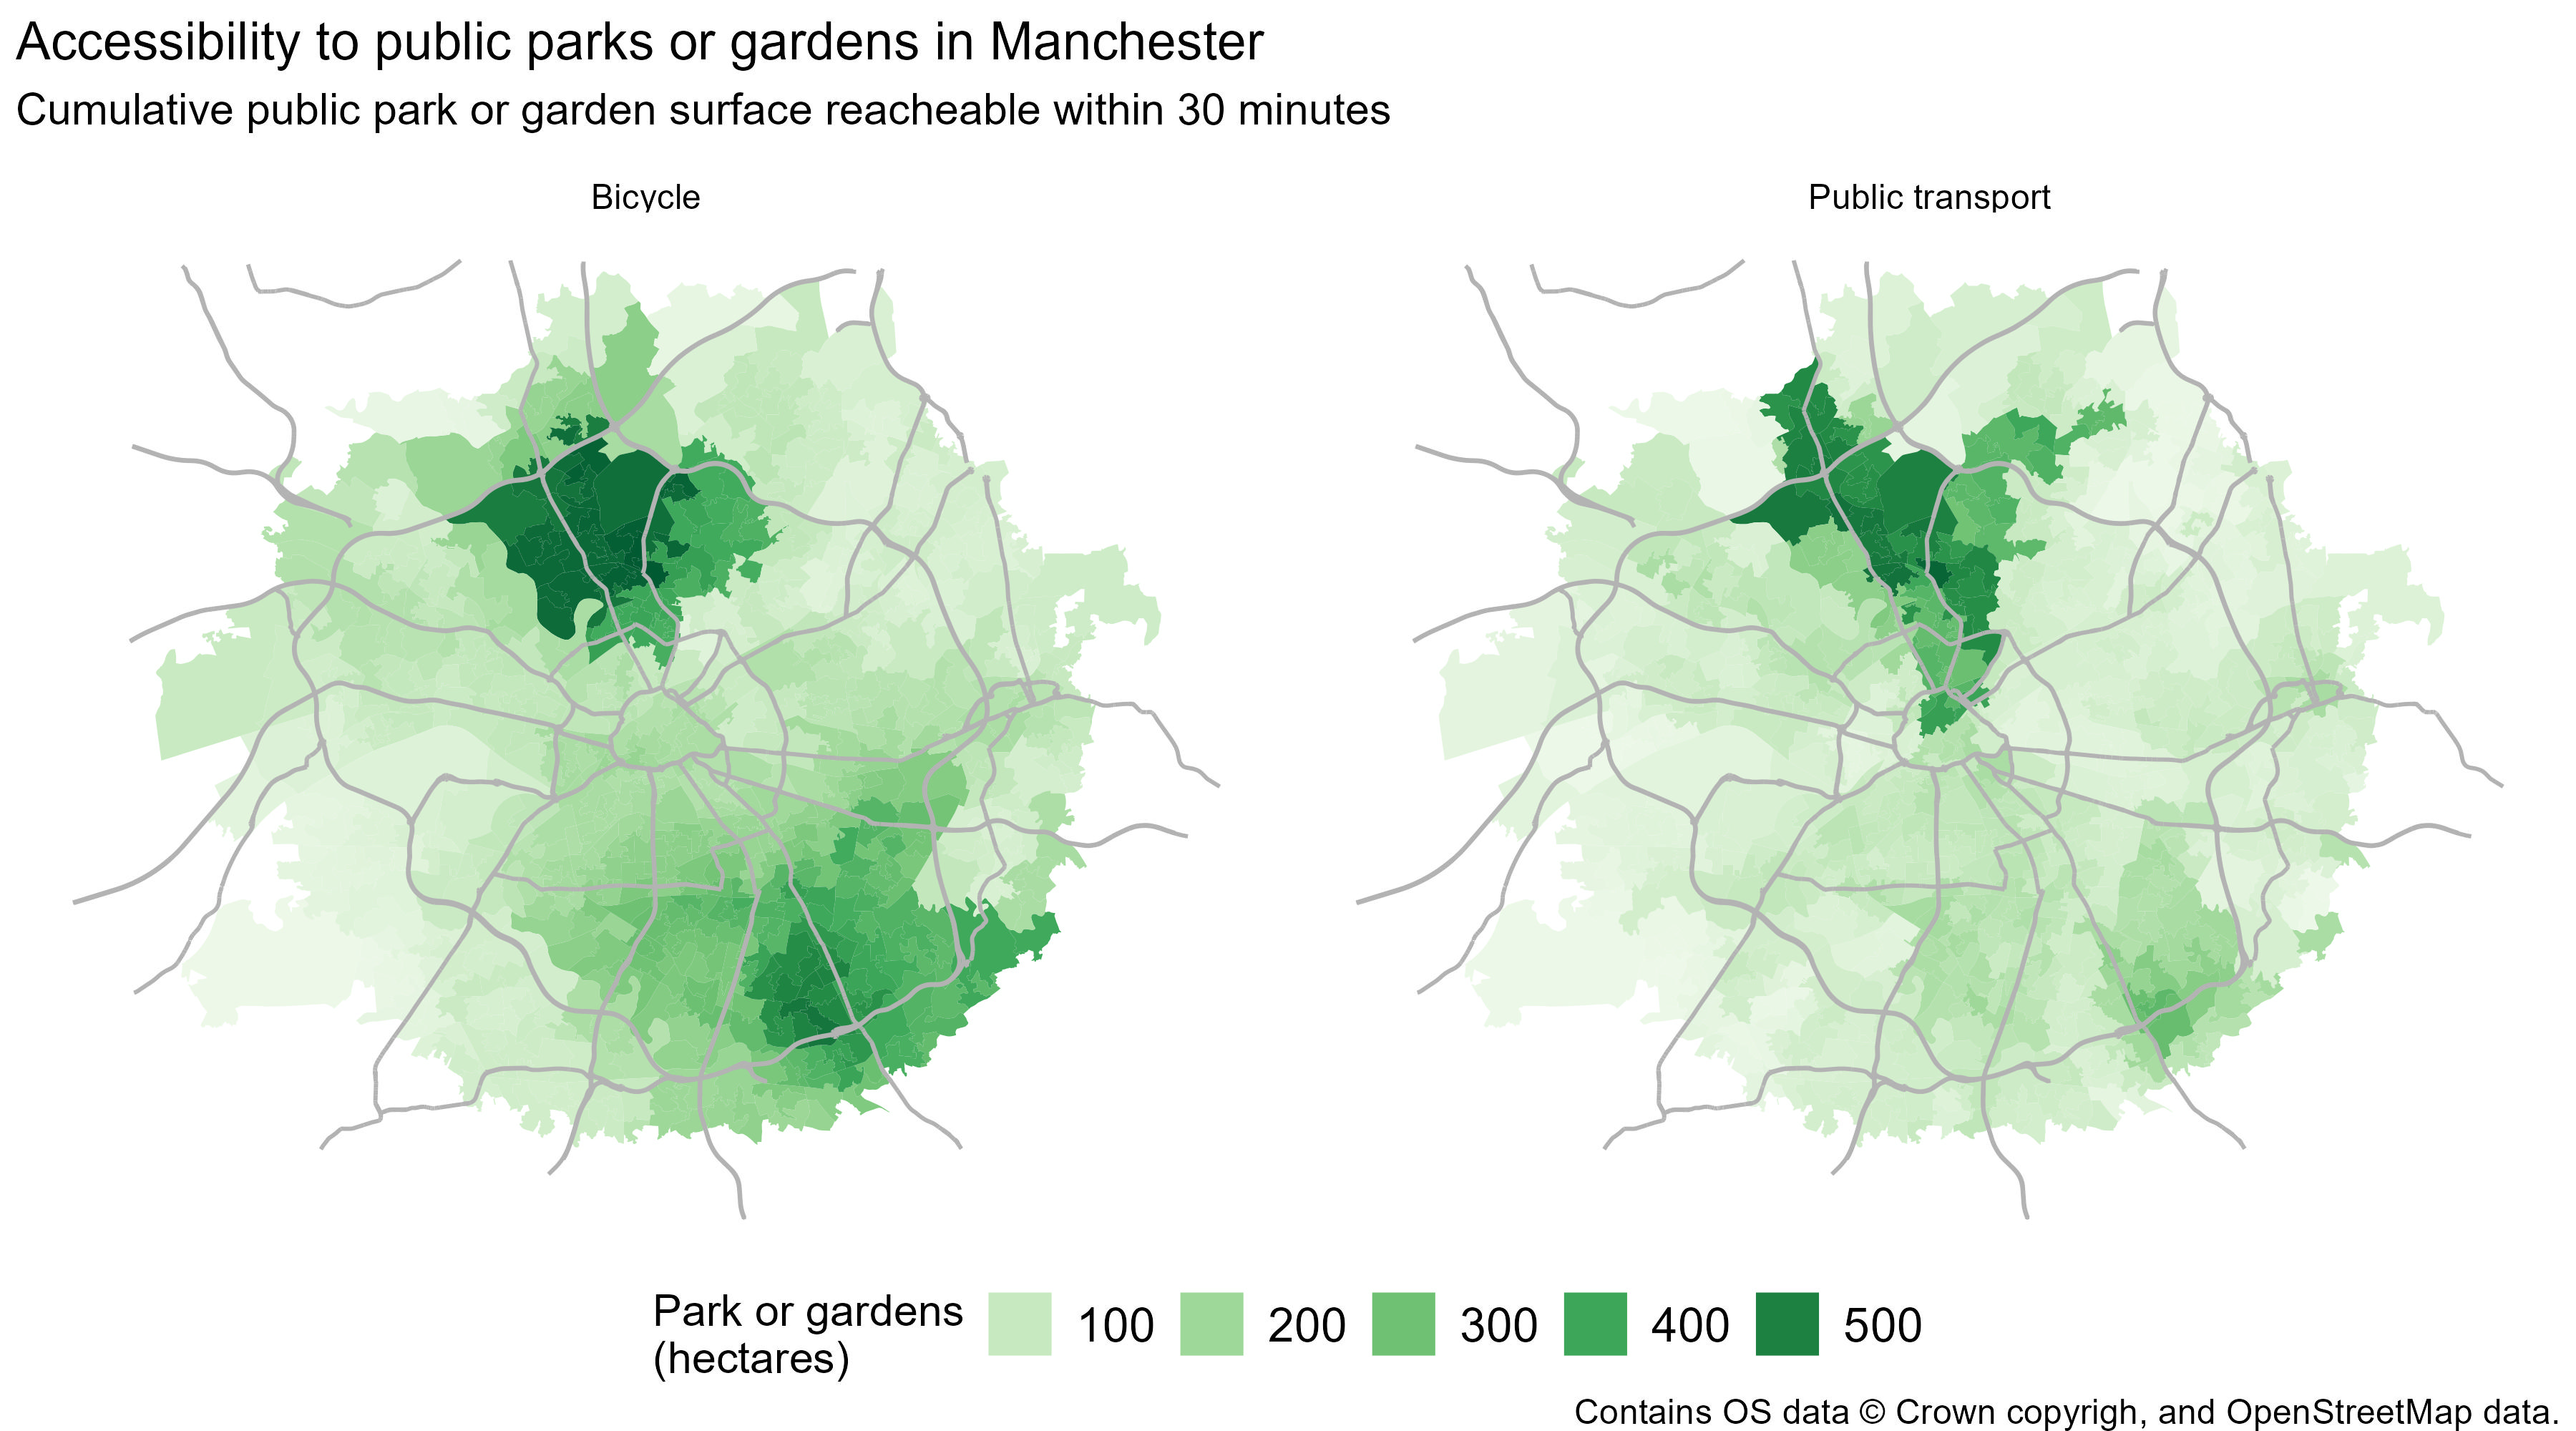
\includegraphics[width=0.9\textwidth]{../plots/parks_map.jpg}
  \caption{Accessibility to public parks or gardens in Manchester area within 30 minutes by bicycle and public transport.}
  \footnotesize{\textit{Source:} the author based on AI23 dataset. Contains OS and OSM data.}
  \label{fig:access-parks}
\end{figure}

\hypertarget{usage-notes}{%
\section{Usage notes}\label{usage-notes}}

The accessibility indicators contained in this dataset are devised for
seamless integration into diverse analyses, facilitated by their
alignment with an official small-area definition. They can be directly
merged with other datasets at the same granularity using the `geo\_code'
identifier in standard software such as Microsoft Excel or comparable
spreadsheet programs. This feature is particularly useful for assessing
the actual reach of essential public services, like health and
education, of distinct population segments, including vulnerable groups.

Additionally, the AI23 can be directly compared with the PTAI22 for
public transport, opening up a range of possibilities for planning
authorities and transport agencies to assess performance. For example,
this can be useful for examining a variety of modifications ranging from
simple operational adjustments such as frequencies to the
introduction/discontinuation of services or physical modifications of
the infrastructure. This is relevant for addressing questions such as
the number of population benefited or affected, or the additional number
of public services covered by public transport.

In addition to LSOA/DZ level analyses, the indicators can be aggregated
at larger geographical units using the \texttt{lookup} file offered by
the InFuse service
(\url{https://infuse.ukdataservice.ac.uk/help/definitions/2011geographies/index.html}).
This includes a hierarchical correspondence to mid areal unit
boundaries, local authority, or region, for example.

The AI23 dataset is also valuable for conducting comparisons between
sustainable transport modes. For instance, the indicators included can
be used to identify communities that have the potential to increase
bicycle usage by demonstrating the mode's effectiveness relative to more
conventional forms, such as public transport. Figure
\ref{fig:bike-comparison} exemplifies this for London for two time cuts,
namely 30 and 45 minutes. The comparison reveals a considerable number
of zones where accessibility to employment by bicycle within 30 minutes
is competitive with that of public transport. The right-hand side panel
shows that there are noticeably more locations with higher accessibility
levels by public transport. Such inputs can be instrumental for
informing demand management strategies by identifying target populations
that could shift to or increase their bicycle usage, especially in areas
where the public transport network experiences peak period congestion.
Additionally, these insights can guide modal integration policies,
favoring the development of bicycle infrastructure when it presents as a
more cost-effective option than expanding public transport.

\begin{figure}[!htbp]
  \centering
  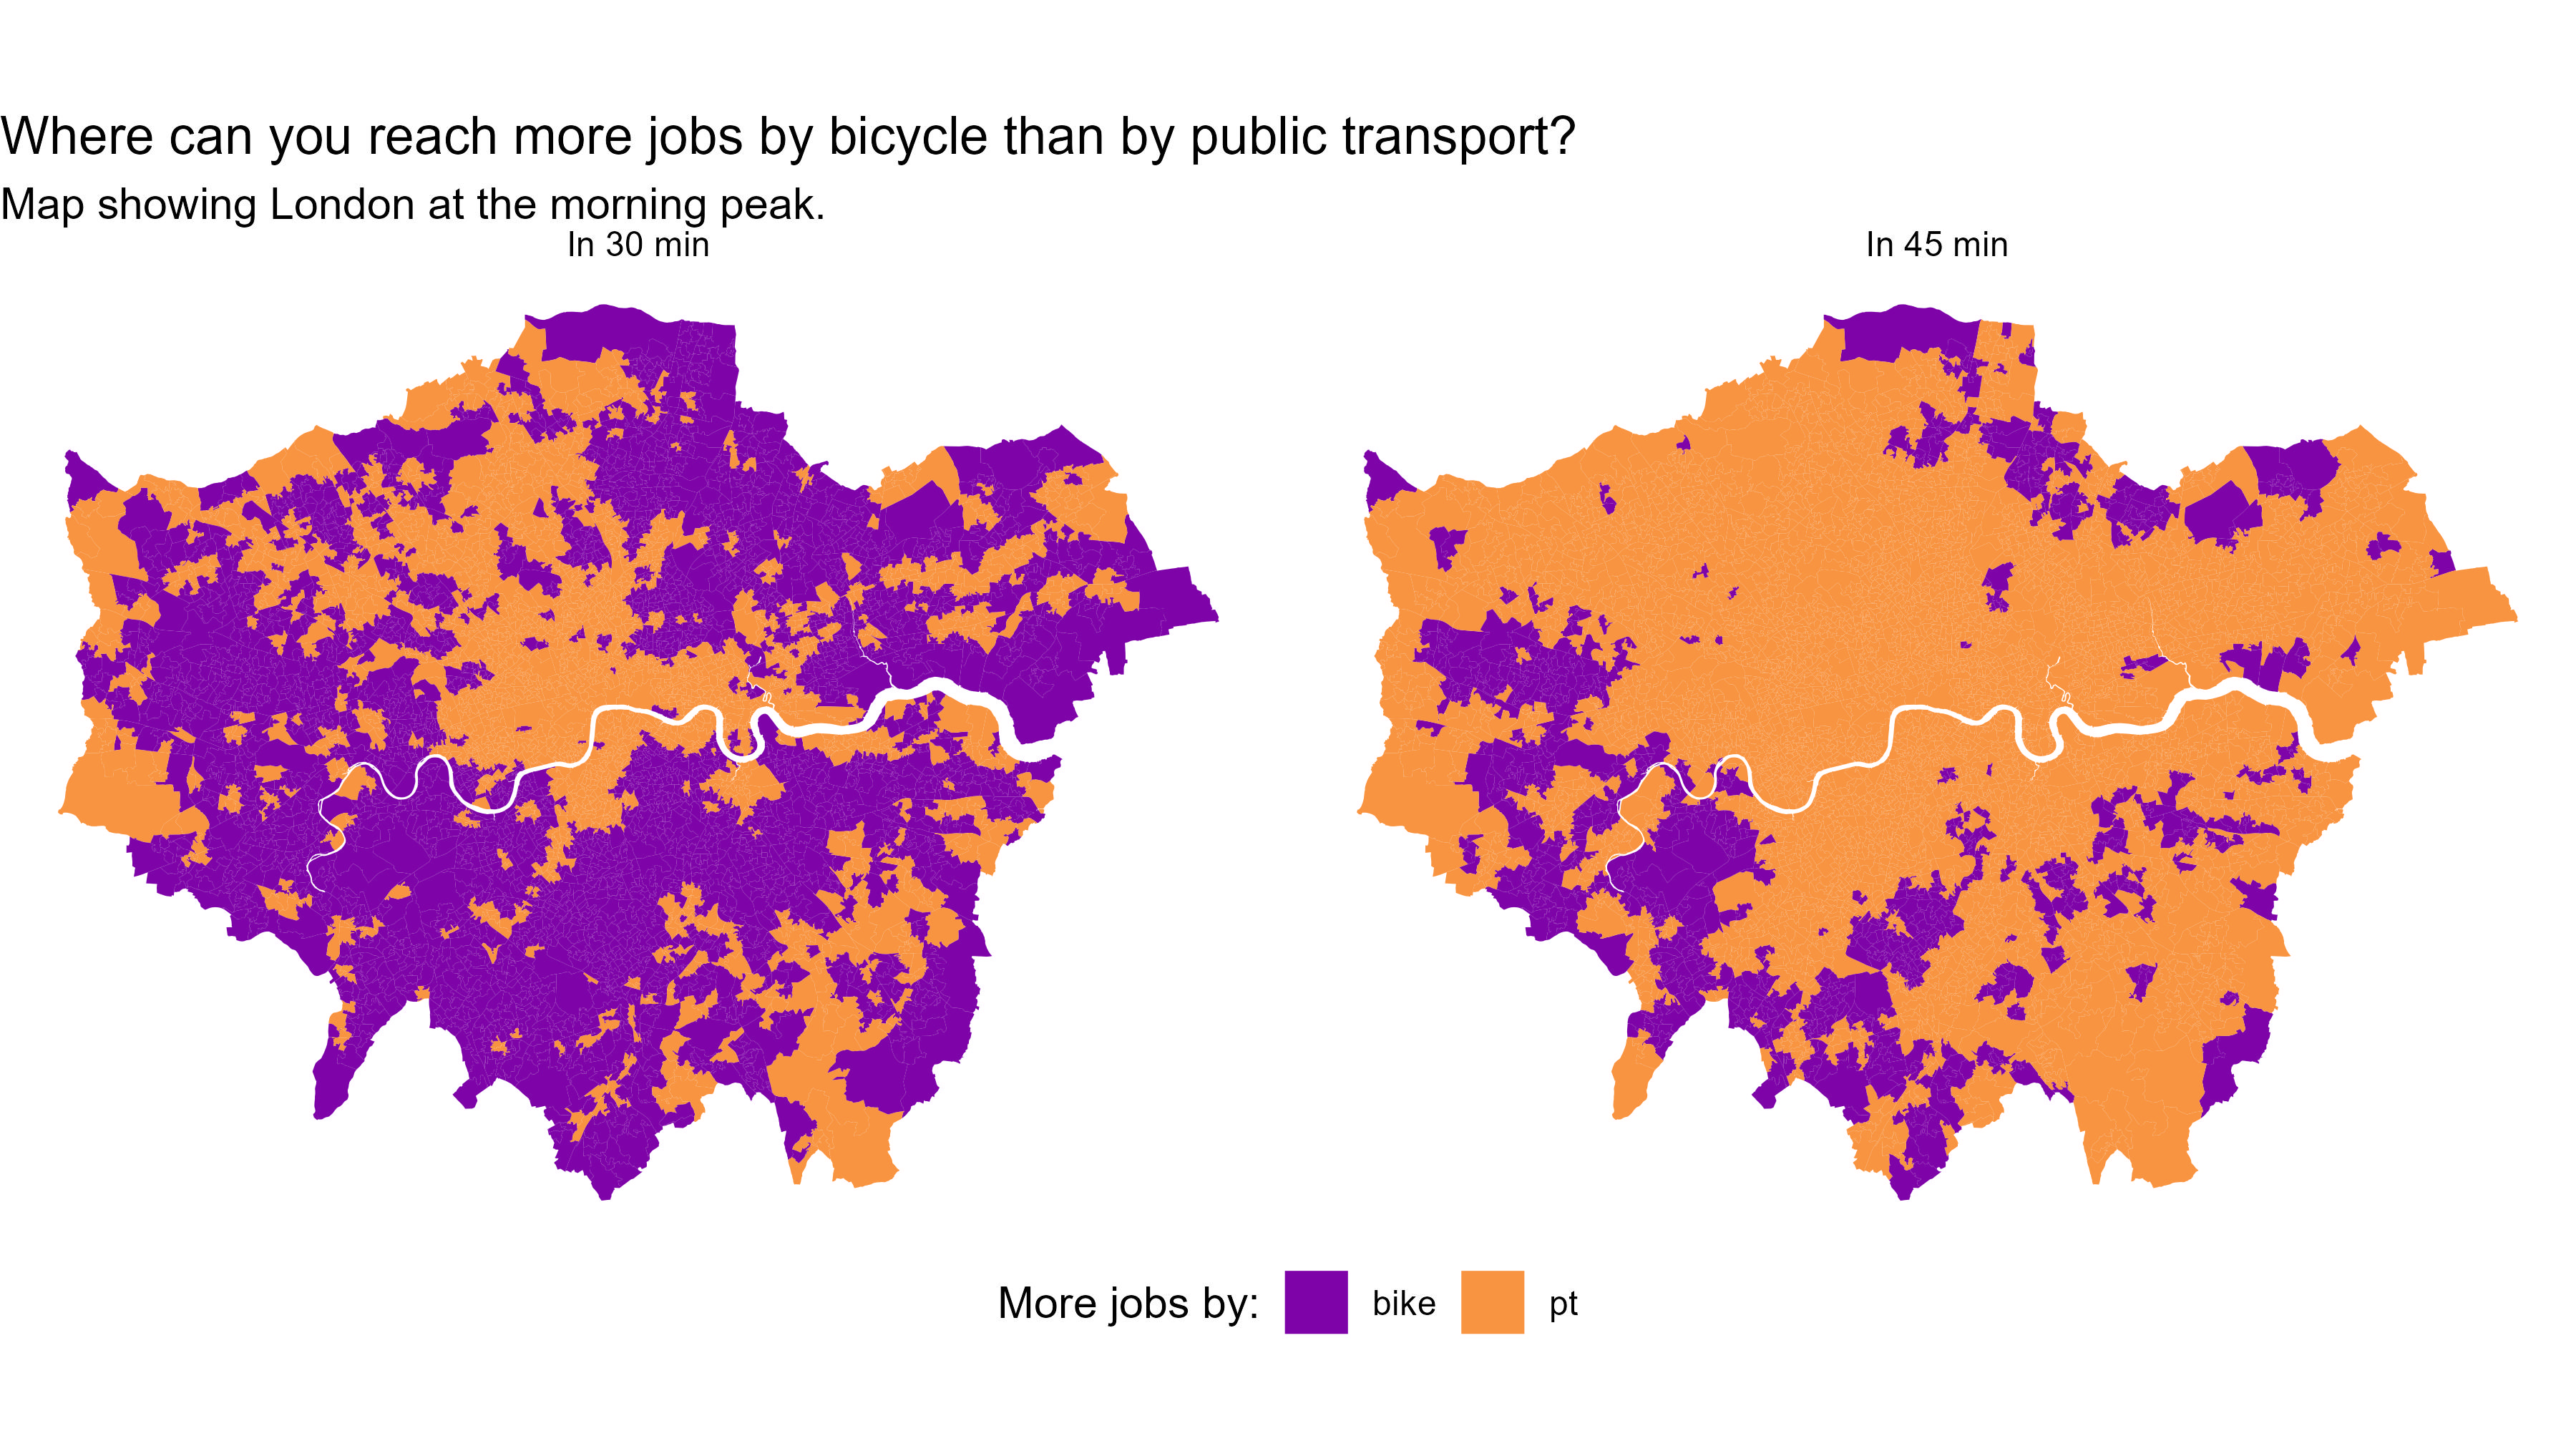
\includegraphics[width=0.9\textwidth]{../plots/pt_vs_bike_map}
  \caption{Accessibiility to employment comparison between bicycle and public transport in London.}
  \footnotesize{\textit{Source:} the author based on AI23 dataset.}
  \label{fig:bike-comparison}
\end{figure}

\pagebreak

\hypertarget{code-availability}{%
\section*{Code availability}\label{code-availability}}
\addcontentsline{toc}{section}{Code availability}

All the code used to generate this data set is openly available in the
following GitHub repository:
\url{https://github.com/urbanbigdatacentre/accessibility_indices23}.

\hypertarget{acknowledgement}{%
\section*{Acknowledgement}\label{acknowledgement}}
\addcontentsline{toc}{section}{Acknowledgement}

This work was made possible by ESRC's on-going support for the Urban Big
Data Centre {[}ES/L011921/1 and ES/S007105/1{]}.

\hypertarget{inventory}{%
\section{Appendix 1. Inventory of files}\label{inventory}}

\begingroup\fontsize{8}{10}\selectfont

\begin{longtable}[t]{>{\raggedright\arraybackslash}p{13cm}ll}
\caption{\label{tab:unnamed-chunk-6}Inventory of files}\\
\toprule
Path & Type & Size\\
\midrule
\endfirsthead
\caption[]{Inventory of files \textit{(continued)}}\\
\toprule
Path & Type & Size\\
\midrule
\endhead

\endfoot
\bottomrule
\endlastfoot
./employment\_accommodation\_9 & directory & 0\\
./employment\_accommodation\_9/access\_employment\_accommodation\_9\_bicycle.csv & file & 4.5M\\
./employment\_accommodation\_9/access\_employment\_accommodation\_9\_pt.csv & file & 8.97M\\
./employment\_accommodation\_9/access\_employment\_accommodation\_9\_walk.csv & file & 4.26M\\
./employment\_agriculture\_1 & directory & 0\\
\addlinespace
./employment\_agriculture\_1/access\_employment\_agriculture\_1\_bicycle.csv & file & 3.47M\\
./employment\_agriculture\_1/access\_employment\_agriculture\_1\_pt.csv & file & 6.82M\\
./employment\_agriculture\_1/access\_employment\_agriculture\_1\_walk.csv & file & 3.06M\\
./employment\_all & directory & 0\\
./employment\_all/access\_employment\_all\_bicycle.csv & file & 4.87M\\
\addlinespace
./employment\_all/access\_employment\_all\_pt.csv & file & 9.71M\\
./employment\_all/access\_employment\_all\_walk.csv & file & 4.64M\\
./employment\_arts\_18 & directory & 0\\
./employment\_arts\_18/access\_employment\_arts\_18\_bicycle.csv & file & 4.42M\\
./employment\_arts\_18/access\_employment\_arts\_18\_pt.csv & file & 8.81M\\
\addlinespace
./employment\_arts\_18/access\_employment\_arts\_18\_walk.csv & file & 4.17M\\
./employment\_business\_14 & directory & 0\\
./employment\_business\_14/access\_employment\_business\_14\_bicycle.csv & file & 4.48M\\
./employment\_business\_14/access\_employment\_business\_14\_pt.csv & file & 8.93M\\
./employment\_business\_14/access\_employment\_business\_14\_walk.csv & file & 4.23M\\
\addlinespace
./employment\_construction\_4 & directory & 0\\
./employment\_construction\_4/access\_employment\_construction\_4\_bicycle.csv & file & 4.45M\\
./employment\_construction\_4/access\_employment\_construction\_4\_pt.csv & file & 8.85M\\
./employment\_construction\_4/access\_employment\_construction\_4\_walk.csv & file & 4.23M\\
./employment\_education\_16 & directory & 0\\
\addlinespace
./employment\_education\_16/access\_employment\_education\_16\_bicycle.csv & file & 4.51M\\
./employment\_education\_16/access\_employment\_education\_16\_pt.csv & file & 8.98M\\
./employment\_education\_16/access\_employment\_education\_16\_walk.csv & file & 4.28M\\
./employment\_financial\_11 & directory & 0\\
./employment\_financial\_11/access\_employment\_financial\_11\_bicycle.csv & file & 4.14M\\
\addlinespace
./employment\_financial\_11/access\_employment\_financial\_11\_pt.csv & file & 8.3M\\
./employment\_financial\_11/access\_employment\_financial\_11\_walk.csv & file & 3.82M\\
./employment\_health\_17 & directory & 0\\
./employment\_health\_17/access\_employment\_health\_17\_bicycle.csv & file & 4.56M\\
./employment\_health\_17/access\_employment\_health\_17\_pt.csv & file & 9.06M\\
\addlinespace
./employment\_health\_17/access\_employment\_health\_17\_walk.csv & file & 4.32M\\
./employment\_information\_10 & directory & 0\\
./employment\_information\_10/access\_employment\_information\_10\_bicycle.csv & file & 4.3M\\
./employment\_information\_10/access\_employment\_information\_10\_pt.csv & file & 8.6M\\
./employment\_information\_10/access\_employment\_information\_10\_walk.csv & file & 4.03M\\
\addlinespace
./employment\_manufacturing\_3 & directory & 0\\
./employment\_manufacturing\_3/access\_employment\_manufacturing\_3\_bicycle.csv & file & 4.43M\\
./employment\_manufacturing\_3/access\_employment\_manufacturing\_3\_pt.csv & file & 8.74M\\
./employment\_manufacturing\_3/access\_employment\_manufacturing\_3\_walk.csv & file & 4.18M\\
./employment\_mining\_2 & directory & 0\\
\addlinespace
./employment\_mining\_2/access\_employment\_mining\_2\_bicycle.csv & file & 4.04M\\
./employment\_mining\_2/access\_employment\_mining\_2\_pt.csv & file & 7.97M\\
./employment\_mining\_2/access\_employment\_mining\_2\_walk.csv & file & 3.73M\\
./employment\_motor\_5 & directory & 0\\
./employment\_motor\_5/access\_employment\_motor\_5\_bicycle.csv & file & 4.24M\\
\addlinespace
./employment\_motor\_5/access\_employment\_motor\_5\_pt.csv & file & 8.38M\\
./employment\_motor\_5/access\_employment\_motor\_5\_walk.csv & file & 4M\\
./employment\_professional\_13 & directory & 0\\
./employment\_professional\_13/access\_employment\_professional\_13\_bicycle.csv & file & 4.48M\\
./employment\_professional\_13/access\_employment\_professional\_13\_pt.csv & file & 8.94M\\
\addlinespace
./employment\_professional\_13/access\_employment\_professional\_13\_walk.csv & file & 4.24M\\
./employment\_property\_12 & directory & 0\\
./employment\_property\_12/access\_employment\_property\_12\_bicycle.csv & file & 4.23M\\
./employment\_property\_12/access\_employment\_property\_12\_pt.csv & file & 8.45M\\
./employment\_property\_12/access\_employment\_property\_12\_walk.csv & file & 3.96M\\
\addlinespace
./employment\_public\_15 & directory & 0\\
./employment\_public\_15/access\_employment\_public\_15\_bicycle.csv & file & 4.26M\\
./employment\_public\_15/access\_employment\_public\_15\_pt.csv & file & 8.46M\\
./employment\_public\_15/access\_employment\_public\_15\_walk.csv & file & 3.94M\\
./employment\_retail\_7 & directory & 0\\
\addlinespace
./employment\_retail\_7/access\_employment\_retail\_7\_bicycle.csv & file & 4.52M\\
./employment\_retail\_7/access\_employment\_retail\_7\_pt.csv & file & 9.01M\\
./employment\_retail\_7/access\_employment\_retail\_7\_walk.csv & file & 4.29M\\
./employment\_transport\_8 & directory & 0\\
./employment\_transport\_8/access\_employment\_transport\_8\_bicycle.csv & file & 4.37M\\
\addlinespace
./employment\_transport\_8/access\_employment\_transport\_8\_pt.csv & file & 8.67M\\
./employment\_transport\_8/access\_employment\_transport\_8\_walk.csv & file & 4.11M\\
./employment\_wholesale\_6 & directory & 0\\
./employment\_wholesale\_6/access\_employment\_wholesale\_6\_bicycle.csv & file & 4.31M\\
./employment\_wholesale\_6/access\_employment\_wholesale\_6\_pt.csv & file & 8.54M\\
\addlinespace
./employment\_wholesale\_6/access\_employment\_wholesale\_6\_walk.csv & file & 4.04M\\
./gp\_practices & directory & 0\\
./gp\_practices/access\_gp\_practices\_bicycle.csv & file & 3.78M\\
./gp\_practices/access\_gp\_practices\_pt.csv & file & 7.49M\\
./gp\_practices/access\_gp\_practices\_walk.csv & file & 3.54M\\
\addlinespace
./hospitals & directory & 0\\
./hospitals/access\_hospitals\_bicycle.csv & file & 3.39M\\
./hospitals/access\_hospitals\_pt.csv & file & 6.68M\\
./hospitals/access\_hospitals\_walk.csv & file & 3.07M\\
./inventory.csv & file & 6.64K\\
\addlinespace
./main\_bua & directory & 0\\
./main\_bua/access\_main\_bua\_bicycle.csv & file & 2.82M\\
./main\_bua/access\_main\_bua\_pt.csv & file & 5.89M\\
./main\_bua/access\_main\_bua\_walk.csv & file & 2.43M\\
./parks & directory & 0\\
\addlinespace
./parks/access\_parks\_bicycle.csv & file & 8.45M\\
./parks/access\_parks\_pt.csv & file & 16.67M\\
./parks/access\_parks\_walk.csv & file & 8.22M\\
./pharmacies & directory & 0\\
./pharmacies/access\_pharmacies\_bicycle.csv & file & 4M\\
\addlinespace
./pharmacies/access\_pharmacies\_pt.csv & file & 7.9M\\
./pharmacies/access\_pharmacies\_walk.csv & file & 3.83M\\
./primary\_schools & directory & 0\\
./primary\_schools/access\_primary\_schools\_bicycle.csv & file & 3.94M\\
./primary\_schools/access\_primary\_schools\_pt.csv & file & 7.78M\\
\addlinespace
./primary\_schools/access\_primary\_schools\_walk.csv & file & 3.72M\\
./secondary\_schools & directory & 0\\
./secondary\_schools/access\_secondary\_schools\_bicycle.csv & file & 3.63M\\
./secondary\_schools/access\_secondary\_schools\_pt.csv & file & 7.13M\\
./secondary\_schools/access\_secondary\_schools\_walk.csv & file & 3.37M\\
\addlinespace
./sub\_bua & directory & 0\\
./sub\_bua/access\_sub\_bua\_bicycle.csv & file & 3.16M\\
./sub\_bua/access\_sub\_bua\_pt.csv & file & 6.35M\\
./sub\_bua/access\_sub\_bua\_walk.csv & file & 2.79M\\
./supermarkets & directory & 0\\
\addlinespace
./supermarkets/access\_supermarkets\_bicycle.csv & file & 3.72M\\
./supermarkets/access\_supermarkets\_pt.csv & file & 7.35M\\
./supermarkets/access\_supermarkets\_walk.csv & file & 3.48M\\
./variable\_descriptor.csv & file & 2.29K\\*
\end{longtable}
\endgroup{}

\hypertarget{references}{%
\section*{References}\label{references}}
\addcontentsline{toc}{section}{References}

\hypertarget{refs}{}
\begin{CSLReferences}{1}{0}
\leavevmode\vadjust pre{\hypertarget{ref-Bastiaanssen2022}{}}%
Bastiaanssen, Jeroen, Daniel Johnson, and Karen Lucas. 2022. {``Does
Better Job Accessibility Help People Gain Employment? {The} Role of
Public Transport in {Great Britain}.''} \emph{Urban Studies} 59 (2):
301--22. \url{https://doi.org/10.1177/00420980211012635}.

\leavevmode\vadjust pre{\hypertarget{ref-Cavallaro2023}{}}%
Cavallaro, Federico, Francesco Bruzzone, and Silvio Nocera. 2023.
{``Effects of High-Speed Rail on Regional Accessibility.''}
\emph{Transportation} 50 (5): 1685--1721.
\url{https://doi.org/10.1007/s11116-022-10291-y}.

\leavevmode\vadjust pre{\hypertarget{ref-Chen2023}{}}%
Chen, Huanfa, Yanjia Cao, Lingru Feng, Qunshan Zhao, and J Rafael
Verduzco Torres. 2023. {``Understanding the Spatial Heterogeneity of
{COVID-19} Vaccination Uptake in {England}.''} \emph{BMC Public Health}
23 (1): 895. \url{https://doi.org/10.1186/s12889-023-15801-w}.

\leavevmode\vadjust pre{\hypertarget{ref-Levinson2020}{}}%
Levinson, David M, and Hao Wu. 2020. {``Towards a General Theory of
Access.''} \emph{Journal of Transport and Land Use} 13 (1): 129--58.
\url{https://doi.org/10.5198/jtlu.2020.1660}.

\leavevmode\vadjust pre{\hypertarget{ref-R-r5r}{}}%
Saraiva, Marcus, Rafael H. M. Pereira, Daniel Herszenhut, Carlos Kaue
Vieira Braga, and Matthew Wigginton Conway. 2021. \emph{R5r: {Rapid}
Realistic Routing with {R5}}. Manual.

\leavevmode\vadjust pre{\hypertarget{ref-VerduzcoTorres2023}{}}%
Verduzco Torres, J Rafael. 2023a. {``Revisiting the Capitalization of
Public Transport Accessibility into Residential Land Value: An Empirical
Analysis Drawing on {Open Science}.''} PhD thesis, {Glasgow}: University
of Glasgow.

\leavevmode\vadjust pre{\hypertarget{ref-VerduzcoTorres2023a}{}}%
---------. 2023b. {``{AccessUK}.''} {Glasgow}: University of Glasgow.

\leavevmode\vadjust pre{\hypertarget{ref-VerduzcoTorres2022}{}}%
Verduzco Torres, J Rafael, and David McArthur. 2022. {``Accessibility
{Indicators} for {Great Britain}.''} Preprint. {Zotero}.
\url{https://doi.org/10.5281/zenodo.6759240}.

\end{CSLReferences}

\bibliographystyle{unsrt}
\bibliography{references.bib}


\end{document}
